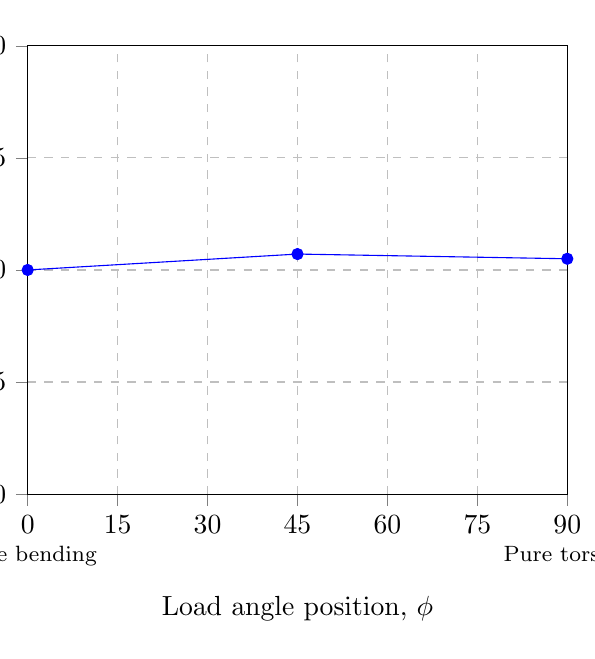
\begin{tikzpicture}[trim axis left, trim axis right]
    \begin{axis}[
        set layers,
        axis line style={on layer=axis foreground},
        grid=both,
        grid style=dashed,
        xtick align=outside,
        ytick align=outside,
        ytick pos=left,
        xtick pos=left,
        ymin=0,
        xmin=0,
        ymax=2.0,
        xmax=90,
        xtick={0,15,...,90},
        xticklabel=$\pgfmathprintnumber{\tick}\si{\degree}$,
        extra x ticks = {0, 90},
        extra x tick labels={Pure bending, Pure torsion},
        every extra x tick/.style={tick label style={anchor=north,yshift=-11pt,font=\footnotesize}},
        ytick={0,0.5,...,2.0},
        xlabel={Load angle position, $\phi$},
        ylabel style={align=center},
        ylabel=Mean yield limit with\\referenceto pure bending,
        y tick label style={
            /pgf/number format/fixed,
            /pgf/number format/fixed zerofill,
            /pgf/number format/precision=1
        }]
    \addplot[color=blue, mark=*, thin] coordinates {
        (0, 1) (45, 1.071) (90, 1.05)};
    \end{axis}   
\end{tikzpicture}